\documentclass{standalone}
\usepackage{tikz}

\begin{document}

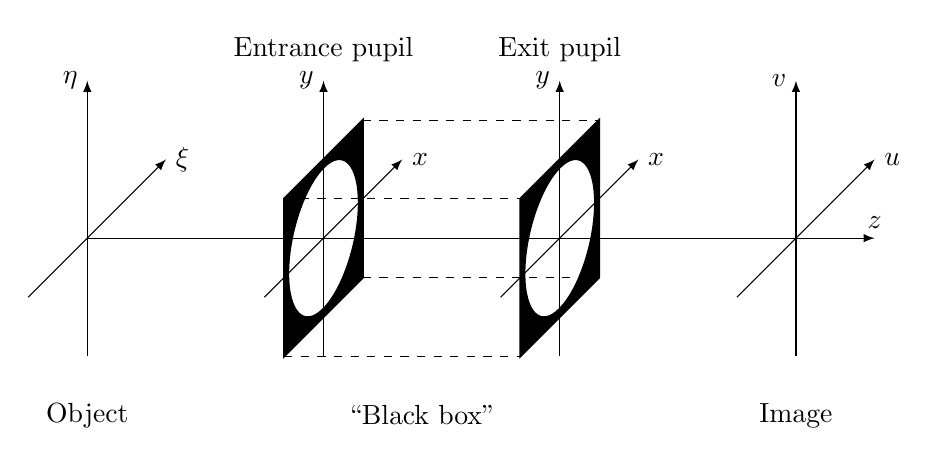
\begin{tikzpicture}[z={(1cm,0cm)},x={(0.5cm,0.5cm)}, y={(0cm,1cm)}, scale=1]
    

    % object
    \coordinate (0) at (0,0,-2);
    
    \draw[-latex] (0) -- +(2,0,0) node [right] {$\xi$};
    \draw (0) -- +(-1.5,0,0);
    
    \draw[-latex] (0) -- +(0,2,0) node [left] {$\eta$};
    \draw (0) -- +(0,-1.5,0);

    \draw[-latex] (0) -- +(0,0,10) node [above] {$z$};
   
    \node [align=left] at (0,-2.25,-2) {Object};
    
    % entrance pupil
    \coordinate (1) at (0,0,1);
    
    \draw[-latex] (1) -- +(2,0,0) node [right] {$x$};
    \draw (1) -- +(-1.5,0,0);
    
    \draw[-latex] (1) -- +(0,2,0) node [left] {$y$};
    \draw (1) -- +(0,-1.5,0);

    \draw [thick, fill=black, even odd rule] 
        (-1,-1,1) -- (1,-1,1) -- (1,1,1) -- (-1,1,1) -- cycle 
        (0,0,1) circle[radius=0.9]; 
    \node [align=left] at (0,2.4,1) {Entrance pupil};


    % exit pupil
    \coordinate (2) at (0,0,4);
    
    \draw[-latex] (2) -- +(2,0,0) node [right] {$x$};
    \draw (2) -- +(-1.5,0,0);
    
    \draw[-latex] (2) -- +(0,2,0) node [left] {$y$};
    \draw (2) -- +(0,-1.5,0);
    
    \draw [thick, fill=black, even odd rule] 
        (-1,-1,4) -- (1,-1,4) -- (1,1,4) -- (-1,1,4) -- cycle 
        (0,0,4) circle[radius=0.9]; 
    \node [align=left] at (0,2.4,4) {Exit pupil};

    % black box
    \draw[dashed] (-1,-1,1) -- (-1,-1,4);
    \draw[dashed] (1,-1,1) -- (1,-1,4);
    \draw[dashed] (1,1,1) -- (1,1,4);
    \draw[dashed] (-1,1,1) -- (-1,1,4);
    \node [align=left] at (0,-2.25,2.25) {``Black box''};
    
    % image
    \coordinate (3) at (0,0,7);
    \draw[-latex] (3) -- +(2,0,0) node [right] {$u$};
    \draw (3) -- +(-1.5,0,0);
    \draw[-latex] (3) -- +(0,2,0) node [left] {$v$};
    \draw (3) -- +(0,-1.5,0);

    \node [align=left] at (0,-2.25,7) {Image};

\end{tikzpicture}

\end{document}
